% !TEX TS-program = XeLaTeX
% use the following command:
% all document files must be coded in UTF-8
\documentclass[portuguese]{textolivre}
% build HTML with: make4ht -e build.lua -c textolivre.cfg -x -u article "fn-in,svg,pic-align"

\usepackage{nameref}

\journalname{Texto Livre}
\thevolume{18}
%\thenumber{1} % old template
\theyear{2025}
\receiveddate{\DTMdisplaydate{2025}{4}{15}{-1}} % YYYY MM DD
\accepteddate{\DTMdisplaydate{2025}{6}{25}{-1}}
\publisheddate{\today}
\corrauthor{Conrado Moreira Mendes}
\articledoi{10.1590/1983-3652.2025.58644}
%\articleid{NNNN} % if the article ID is not the last 5 numbers of its DOI, provide it using \articleid{} commmand 
% list of available sesscions in the journal: articles, dossier, reports, essays, reviews, interviews, editorial
\articlesessionname{articles}
\runningauthor{Mendes, Almeida e Mattos} 
%\editorname{Leonardo Araújo} % old template
\sectioneditorname{Daniervelin Pereira}
\layouteditorname{Saula Cecília}

\title{Ecossistema desinformacional em canais de extrema-direita no Telegram sobre as enchentes no RS em 2024: abordagem semiótico-interacional}
\othertitle{Disinformation ecosystem in far-right Telegram channels about the 2024 floods in Rio Grande do Sul: a sociosemiotic-interactional approach}
% if there is a third language title, add here:
%\othertitle{Artikelvorlage zur Einreichung beim Texto Livre Journal}

\author[1]{Conrado Moreira Mendes~\orcid{0000-0002-3721-8578}\thanks{Email: \href{mailto:conradomendes@yahoo.com.br}{conradomendes@yahoo.com.br}}}
\author[1]{Carolina Gouvêa de Almeida~\orcid{0009-0009-5442-9850}\thanks{Email: \href{mailto:carolcgalmeida@gmail.com}{carolcgalmeida@gmail.com}}}
\author[1]{Maria Ângela Mattos~\orcid{0000-0002-0764-6846}\thanks{Email: \href{mailto:mattos.maria.angela@gmail.com}{mattos.maria.angela@gmail.com}}}
\affil[1]{Pontifícia Universidade Católica de Minas Gerais, Belo Horizonte, MG, Brasil.}


\addbibresource{article.bib}
% use biber instead of bibtex
% $ biber article

% used to create dummy text for the template file
\definecolor{dark-gray}{gray}{0.35} % color used to display dummy texts
\usepackage{lipsum}
\SetLipsumParListSurrounders{\colorlet{oldcolor}{.}\color{dark-gray}}{\color{oldcolor}}

% used here only to provide the XeLaTeX and BibTeX logos
\usepackage{hologo}

% if you use multirows in a table, include the multirow package
\usepackage{multirow}

% provides sidewaysfigure environment
\usepackage{rotating}

% CUSTOM EPIGRAPH - BEGIN 
%%% https://tex.stackexchange.com/questions/193178/specific-epigraph-style
\usepackage{epigraph}
\renewcommand\textflush{flushright}
\makeatletter
\newlength\epitextskip
\pretocmd{\@epitext}{\em}{}{}
\apptocmd{\@epitext}{\em}{}{}
\patchcmd{\epigraph}{\@epitext{#1}\\}{\@epitext{#1}\\[\epitextskip]}{}{}
\makeatother
\setlength\epigraphrule{0pt}
\setlength\epitextskip{0.5ex}
\setlength\epigraphwidth{.7\textwidth}
% CUSTOM EPIGRAPH - END

% to use IPA symbols in unicode add
%\usepackage{fontspec}
%\newfontfamily\ipafont{CMU Serif}
%\newcommand{\ipa}[1]{{\ipafont #1}}
% and in the text you may use the \ipa{...} command passing the symbols in unicode

% LANGUAGE - BEGIN
% ARABIC
% for languages that use special fonts, you must provide the typeface that will be used
% \setotherlanguage{arabic}
% \newfontfamily\arabicfont[Script=Arabic]{Amiri}
% \newfontfamily\arabicfontsf[Script=Arabic]{Amiri}
% \newfontfamily\arabicfonttt[Script=Arabic]{Amiri}
%
% in the article, to add arabic text use: \textlang{arabic}{ ... }
%
% RUSSIAN
% for russian text we also need to define fonts with support for Cyrillic script
% \usepackage{fontspec}
% \setotherlanguage{russian}
% \newfontfamily\cyrillicfont{Times New Roman}
% \newfontfamily\cyrillicfontsf{Times New Roman}[Script=Cyrillic]
% \newfontfamily\cyrillicfonttt{Times New Roman}[Script=Cyrillic]
%
% in the text use \begin{russian} ... \end{russian}
% LANGUAGE - END

% EMOJIS - BEGIN
% to use emoticons in your manuscript
% https://stackoverflow.com/questions/190145/how-to-insert-emoticons-in-latex/57076064
% using font Symbola, which has full support
% the font may be downloaded at:
% https://dn-works.com/ufas/
% add to preamble:
\newfontfamily\Symbola{Symbola}
% in the text use:
% {\Symbola }
% EMOJIS - END

% LABEL REFERENCE TO DESCRIPTIVE LIST - BEGIN
% reference itens in a descriptive list using their labels instead of numbers
% insert the code below in the preambule:
%\makeatletter
%\let\orgdescriptionlabel\descriptionlabel
%\renewcommand*{\descriptionlabel}[1]{%
%  \let\orglabel\label
%  \let\label\@gobble
%  \phantomsection
%  \edef\@currentlabel{#1\unskip}%
%  \let\label\orglabel
%  \orgdescriptionlabel{#1}%
%}
%\makeatother
%
% in your document, use as illustraded here:
%\begin{description}
%  \item[first\label{itm1}] this is only an example;
%  % ...  add more items
%\end{description}
% LABEL REFERENCE TO DESCRIPTIVE LIST - END


% add line numbers for submission
%\usepackage{lineno}
%\linenumbers

\begin{document}
\maketitle

\begin{polyabstract}
\begin{abstract}
Esta pesquisa teve como objetivo compreender o ecossistema desinformacional em canais públicos de extrema-direita no aplicativo Telegram, com foco nas postagens sobre as enchentes no Rio Grande do Sul (RS) no primeiro semestre de 2024. Foram analisadas 25 postagens selecionadas com base no critério de maior interação, todas veiculadas em canais públicos de extrema-direita. A abordagem teórico-metodológica adotada fundamenta-se na semiótica discursiva e na sociossemiótica. A análise contemplou tanto os conteúdos das postagens quanto as reações em emoji por parte dos inscritos nos canais. Com base nas análises realizadas, foram propostas as seguintes tipologias discursivas do ecossistema desinformacional: conteúdo declaratório, conteúdo enganoso, discurso de ódio, ironia, memes e teorias conspiratórias. Identificaram-se ainda, entre os temas mais recorrentes, críticas à negligência governamental, denúncias de expropriação de terras com motivação ideológica e alegações de que a inação estatal estaria promovendo a morte de civis, entre outros. A pesquisa evidenciou também o uso de emojis como forma condensada de discurso de ódio. Observou-se, por fim, que a adesão à desinformação ocorre não apenas por meio dos contratos fiduciário e veridictório, mas também no interior do regime de ajustamento, com base na interação sensível entre sujeitos.

\keywords{Desinformação\sep Semiótica\sep Canais de extrema-direita\sep Enchentes no Rio Grande do Sul}
\end{abstract}

\begin{english}
\begin{abstract}
 This study aimed to understand the disinformation ecosystem in public far-right channels on the messaging app Telegram, focusing on posts about the floods in Rio Grande do Sul (RS) during the first half of 2024. A total of 25 posts were analyzed, selected based on the criterion of highest engagement, all published in public far-right channels. The theoretical and methodological framework adopted is based on discursive semiotics and sociosemiotics. The analysis considered both the content of the posts and the emoji reactions by channel subscribers. Based on the analyses, the following discursive typologies of the disinformation ecosystem were proposed: declarative content, misleading content, hate speech, irony, memes, and conspiracy theories. Among the most frequent themes were criticisms of governmental negligence, denunciations of ideologically motivated land expropriation, and claims that state inaction was promoting civilian deaths, among others. The study also highlighted the use of emojis as a condensed form of hate speech. Finally, it was observed that adherence to disinformation occurs not only through fiduciary and veridictory contracts but also within the regime of adjustment, based on the sensitive interaction between subjects.

\keywords{Disinformation\sep Semiotics\sep Far-right channels\sep Floods in Rio Grande do Sul (Brazil)}
\end{abstract}
\end{english}
% if there is another abstract, insert it here using the same scheme
\end{polyabstract}

\section{Introdução}
Esta pesquisa analisa postagens sobre as enchentes no Rio Grande do Sul (RS) que circularam em canais públicos de extrema-direita do aplicativo de mensageria Telegram a partir de abordagem teórico-metodológica da semiótica discursiva e da sociossemiótica, com o objetivo de compreender o ecossistema desinformacional nos referidos canais dessa plataforma. As postagens selecionadas foram publicadas no Telegram durante o período de 27 de abril, início das chuvas fortes no Vale do Rio Pardo \cite{bbc2024inundacoes}, a 31 de maio de 2024, correspondendo ao período de maior fluxo de compartilhamento de informações referentes à catástrofe. O \textit{corpus} da pesquisa totalizou 25 postagens. Na análise qualitativa, adotou-se abordagem semiótica, que contemplou o conteúdo das postagens. Com base nas análises realizadas, são propostas, preliminarmente, algumas tipologias discursivas do ecossistema desinformacional. Em seguida, são examinados os principais discursos (temas mais recorrentes) do \textit{corpus} da pesquisa. 

Além desta introdução, o presente artigo conta com uma seção intitulada \nameref{sec-semiotica-desin}, na qual o fenômeno da desinformação é abordado à luz da semiótica e da sociossemiótica. Em seguida, apresenta-se a seção \nameref{sec-metodologia}, dedicada à explicitação dos procedimentos metodológicos de coleta e análise do \textit{corpus}. Na sequência, há uma seção de \nameref{sec-carac_corpus}, com a descrição dos canais analisados, seguida pela seção que trata das \nameref{sec-postagens_recorrentes}. Posteriormente, propõe-se uma \nameref{sec-tipologias-discur} deduzida do \textit{corpus} analisado. Em seguida, dedica-se uma seção à análise dos \nameref{sec-discursos_rec} disseminados no discurso. Por fim, o artigo é encerrado com as \nameref{sec-conclusao}, que retomam os principais achados e apontam para as contribuições desta pesquisa.

\section{Semiótica da desinformação}\label{sec-semiotica-desin}
Segundo \textcite{mendes2025}, a desinformação, à luz da semiótica discursiva, define-se, inicialmente, como texto ou como discurso. No primeiro caso, trata-se de qualquer expressão que veicule um conteúdo, no segundo, de um conteúdo não textualizado. Assim, para o autor, pode-se falar em textos e discursos \emph{desinformacionais}\footnote{O autor prefere utilizar \emph{desinformacional} a \emph{desinformativo}, pois, na tradição dos estudos em Comunicação, o termo \emph{comunicativo} é entendido como transmissão, enquanto o termo \emph{comunicacional} diz respeito à comunicação como interação.}. Portanto, um discurso desinformacional, quando se textualiza, se converte em texto desinformacional. À medida que circulam entre destinadores e destinatários da comunicação, tais textos e discursos são então submetidos aos contratos fiduciário -- associado à crença e veridictório -- relacionado ao seu parecer verdadeiro. Quando há adesão, por parte do destinatário da comunicação a tais contratos, tais textos/discursos passam a ser sancionados como verdadeiros. Com efeito, segundo \textcite{greimas2008}, ambos os contratos estão profundamente inter-relacionados:

\begin{quote}
    Ele [o contrato fiduciário] se manifesta, entretanto, também no nível da estrutura da enunciação e apresenta-se então como um contrato enunciativo [...], ou como contrato de veridicção, já que visa a estabelecer uma convenção fiduciária entre o enunciador e o enunciatário, referindo-se   ao   estatuto   veridictório (ao dizer-verdadeiro) do discurso enunciado. O contrato fiduciário que assim se instaura, pode repousar em uma evidência (isto é, numa certeza imediata) ou então ser precedido de um fazer persuasivo (de um fazer-crer) do enunciador, ao   qual   corresponde   um   fazer interpretativo (um crer) da parte do enunciatário \cite[p. 86, grifos dos autores]{greimas2008}.
\end{quote}

Assim, uma característica constante da desinformação é sua orientação para a produção de um efeito de veridicção, com o objetivo de conquistar a adesão do destinatário. Nesse contexto, conforme apontam \textcite{ribeiro2022}, em leitura comparativa entre Peirce e Greimas aplicada ao fenômeno da desinformação, destaca-se o papel central da crença no processo de sanção da desinformação como um discurso tomado como verdadeiro:

\begin{quote}
    Há uma interseção significativa entre as duas abordagens, que reside no papel que as crenças desempenham nas trocas discursivas e na construção do sentido. De maneira congruente, ambas as perspectivas explicitam que o entendimento da verdade passa por um sistema cognitivo ligado à construção de crenças dos indivíduos Desse modo, pela perspectiva peirciana, a crença é uma espécie de hábito que direciona condutas, mesmo diante de evidências que questionem a sua veracidade. Já pela perspectiva greimasiana, o discurso da desinformação parece obter a sanção fiduciária fundada sobretudo no crer do enunciatário \cite[p. 13]{ribeiro2022}.
\end{quote}

Em proposição recente, para \textcite{landowski2022}, os efeitos de verdade são construídos por interações que não necessariamente se pautam pela noção greimasiana de contrato, o que implica a construção de verdade a partir de outros princípios que não o da intencionalidade, o qual corresponde ao regime de interação e de sentido da manipulação. Para o autor, efeitos de verdade podem ser engendrados considerando-se todos os regimes interacionais, ou seja, a programação, a manipulação, o ajustamento e o acidente, o que permite construir, as verdades provadas, as negociadas, a experimentada e a relevada, respectivamente. 

Portanto, \textcite[p. 8]{mendes2025}, à luz da sociossemiótica, afirma que:

\begin{quote}
    A desinformação é um efeito de verdadeiro que pode ser construído no interior de um regime interacional regido pela inteligibilidade e/ou pela sensibilidade. O primeiro, em estado puro (que existe apenas em teoria), estaria ligado ao debate de ideias entre sujeitos puramente racionais. O segundo, por sua vez, diria respeito à construção de um efeito de verdadeiro a partir do contágio entre sensibilidades.
\end{quote}

O autor, no entanto, pondera ser muito difícil afirmar que o fenômeno da desinformação se baseie apenas em um ou outro regime, mas atenta para uma certa tendência à construção de efeitos de verdade a partir de uma lógica ligada ao regime do ajustamento sensível. \textcite{mendes2025} aponta ainda para uma perspectiva de coparticipação entre regimes, no sentido de que efeitos de verdadeiro que se constroem na articulação entre diferentes regimes de interação. 

Após alguns apontamentos teóricos sobre a concepção semiótica de desinformação, passa-se aos procedimentos metodológicos do trabalho.

\section{Metodologia}\label{sec-metodologia}
Este trabalho desenvolveu uma pesquisa exploratória na plataforma de mensagens Telegram sobre as enchentes do Rio Grande do Sul no primeiro semestre de 2024, estudando cinco canais públicos de extrema-direita. A metodologia, de natureza quantitativa e qualitativa, foi dividida em quatro etapas, a saber: (1) seleção de canais; (2) seleção de postagens; (3) apuração das postagens mais recorrentes e constituição do \textit{corpus} da pesquisa; (4) análise do \textit{corpus} da pesquisa.

As publicações analisadas foram veiculadas no Telegram entre 27 de abril, data marcada pelo início das chuvas intensas no Vale do Rio Pardo \cite{bbc2024inundacoes}, e 31 de maio, intervalo que concentrou o maior volume de circulação de informações relacionadas ao desastre.

Na primeira etapa, foram identificados 20 canais de mensagens que obedeceram a busca pelas seguintes palavras-chave: \emph{Brasil, direita, patriota, pátria, conservador, nação, aliança, aliados}. Dentre eles, foram selecionados os cinco canais com maior número de inscritos que compartilharam desinformação sobre a catástrofe do Rio Grande do Sul como denunciado pela Secom \cite{agenciabrasil2024}:

\begin{quote}
    Têm circulado nos aplicativos de mensageria (Telegram) notícias falsas criticando uma ``falta de atenção'' ao povo do Sul pelo Governo Federal. Usuários estão compartilhando que o Executivo ``foi rápido ao usar avião da FAB para levar 125 toneladas de alimentos a Cuba e essa agilidade não foi utilizada no caso do RS''. Há mensagens criticando a ausência de ministros no Sul do país e condenando a ida da primeira-dama ao Rio de Janeiro para o show da Madonna. As mensagens foram compartilhadas em grupos que reúnem mais de 20 mil pessoas no total.
\end{quote}

São eles, por ordem do número de usuários inscritos:

\begin{enumerate}
    \item O INFORMANTE, com 140.377 inscritos; 
    \item MBL -- Movimento Brasil Livre, com 28.291 inscritos;
    \item Paladin, com 14.392 inscritos;
    \item DIREITA BRASIL, com 12.923 inscritos;
    \item SALDANHA -- Endireitando Brasil, com 4.362 inscritos;
\end{enumerate}
\medskip

Na segunda etapa, foi realizada a seleção manual preliminar de 20 mensagens em cada canal, sendo as 10 mais reagidas e 10 mais comentadas, sobre a temática ``Enchentes do RS'', totalizando 100 mensagens. Na terceira etapa, usou-se o critério de maior interação a partir da soma do número de reações e do número de comentários para constituir o \textit{corpus} da pesquisa, que totalizou 25 postagens.

Após a definição do \textit{corpus}, adotou-se a abordagem da semiótica discursiva e da sociossemiótica para analisar o conteúdo das postagens por meio da análise dos temas, correspondentes à semântica discursiva, e das reações em emoji pelos membros dos canais. A descrição e interpretação dos \textit{emojis} foi retirada do \textit{website} Emojipedia.


\section{Caracterização do \textit{corpus}}\label{sec-carac_corpus}

\subsection{Descrição dos canais}
O canal com maior número de membros é \emph{O Informante}, com 140.377 membros\footnote{Não foi possível identificar os responsáveis pelo canal, devido ao anonimato característico da plataforma Telegram.}. A descrição do canal feita por ele próprio é (\Cref{fig-1}): ``Principais notícias internacionais, coberturas sob perspectiva bíblica. Seja parte também do nosso canal restrito muito mais aprofundado''. A foto de capa (\Cref{fig-2}) é uma peça gráfica representando elementos tecnológicos diversos em azul. No centro, a impressão digital branca de uma mão humana é circulada por uma leve linha vermelha. Abaixo do desenho está escrito o nome, em caixa alta, ``O INFORMANTE''.

%--- CÓDIGO DAS FIGURAS 1 E 2 ---%
\begin{figure}[h!]
    \centering
    % Primeira imagem
    \begin{minipage}{0.45\textwidth}
        \centering
        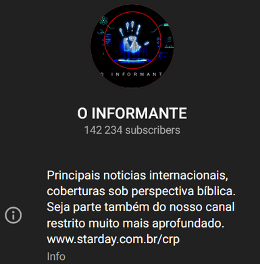
\includegraphics[width=\linewidth]{Imagens/Fig1.png}
        \caption{Descrição do canal \emph{O Informante}.}
        \label{fig-1}
    \end{minipage}
    \hfill
    % Segunda imagem
    \begin{minipage}{0.45\textwidth}
        \centering
        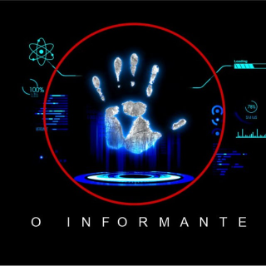
\includegraphics[width=\linewidth]{Imagens/Fig2.png}
        \caption{Foto de capa do canal \emph{O Informante}.}
        \label{fig-2}
    \end{minipage}
    \source{\textcite{telegram2024}.}
\end{figure}

O segundo canal com maior número de membros é o \emph{MBL -- Movimento Brasil Livre}, com 28.291 membros. \emph{MBL -- Movimento Brasil Livre} é o canal oficial do Telegram do movimento conservador de direita ``MBL'', fundado pelo político, ativista e youtuber Kim Kataguiri \cite{gazetadopovo2015}. A descrição do canal no Telegram (\Cref{fig-3}), ``Siga também no WhatsApp'' , leva ao canal correspondente da plataforma de mensagens WhatsApp, que declara: ``Aqui você encontra as principais notícias do movimento, de seus porta-vozes, além de notícias de política e economia do país e do mundo''. Sua foto de capa (\Cref{fig-4}) é a logo do MBL: a bandeira do Brasil vetorizada em formato de seta levando às letras ``MBL'' na cor azul e um fundo de tom mais claro. Em fonte menor está escrito: ``Movimento Brasil Livre''.

%--- CÓDIGO DAS FIGURAS 3 E 4 ---%
\begin{figure}[h!]
    \centering
    % Primeira imagem
    \begin{minipage}[t]{0.35\textwidth}
        \centering
        
\includegraphics[width=\linewidth]{Imagens/Fig3.png}
        \caption{Descrição do canal \emph{MBL -- Movimento Brasil Livre}.}
        \label{fig-3}
        \source{\textcite{telegram2024}.}
    \end{minipage}
    \hfill
    % Segunda imagem
    \begin{minipage}[t]{0.6\textwidth}
        \centering
        
\includegraphics[width=\linewidth]{Imagens/Fig4.png}
        \caption{Descrição do canal \emph{MBL -- Movimento Brasil Livre}.}
        \label{fig-4}
        \source{\textcite{mbl2024whatsapp}.}
    \end{minipage}
\end{figure}

%\newpage
O terceiro canal com maior número de membros é o \emph{Paladin}, com 14.392 membros\footnote{Embora o administrador do canal utilize o pseudônimo \emph{Paladin}, sua identidade real não é divulgada publicamente.}. No contexto medieval, a figura do ``paladino'' é de um ``homem corajoso e cavalheiresco, extremado defensor dos oprimidos e das causas justas'' \cite{michaelis2024}. A descrição do canal (\Cref{fig-5}), ``Escolha o seu caminho'', leva a uma página do Linktree com outras redes sociais associadas ao canal. Sua foto de capa (\Cref{fig-6}) é a imagem, gerada por inteligência artificial, de um homem branco, de expressão sóbria, trajando vestes medievais.

%--- CÓDIGO DAS FIGURAS 5 E 6 ---%
\begin{figure}[h!]
    \centering
    % Primeira imagem
    \begin{minipage}[t]{0.47\textwidth}
        \centering        
\includegraphics[width=\linewidth]{Imagens/Fig5.png}
        \caption{Descrição do canal \emph{Paladin}.}
        \label{fig-5}
    \end{minipage}
    \hfill
    % Segunda imagem
    \begin{minipage}[t]{0.37\textwidth}
        \centering
    
\includegraphics[width=\linewidth]{Imagens/Fig6.png}
        \caption{Foto de capa do canal \emph{Paladin}.}
        \label{fig-6}
    \end{minipage}
    \source{\textcite{telegram2024}.}
\end{figure}

O quarto canal com maior número de membros é o \emph{DIREITA BRASIL}, com 12.923 membros\footnote{Assim como nos casos anteriores, o canal Direita Brasil também é administrado por indivíduos ou grupos que optam pelo anonimato, não tornando pública sua identidade.}. A descrição do canal (\Cref{fig-7}) faz referência a um canal anterior que foi encerrado pela plataforma Telegram: ``Recomeçando! O canal anterior foi bloqueado'', mas não explicita sua temática. Apesar de não constar na descrição, o nome do canal já faz referência ao espectro político, assim como sua foto de capa (\Cref{fig-8}): a imagem da bandeira nacional, que faz alusão a movimentos brasileiros de extrema-direita. 

%--- CÓDIGO DAS FIGURAS 7 E 8 ---%
\begin{figure}[h!]
    \centering
    % Primeira imagem
    \begin{minipage}[t]{0.48\textwidth}
        \centering
        
\includegraphics[width=\linewidth]{Imagens/Fig7.png}
        \caption{Descrição do canal \emph{DIREITA BRASIL}.}
        \label{fig-7}
    \end{minipage}
    \hfill
    % Segunda imagem
    \begin{minipage}[t]{0.44\textwidth}
        \centering
        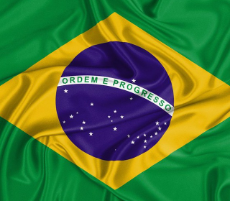
\includegraphics[width=\linewidth]{Imagens/Fig8_1.png}
        \caption{Foto de capa do canal \emph{DIREITA BRASIL}.}
        \label{fig-8}
    \end{minipage}
    \source{\textcite{telegram2024}.}
\end{figure}

Por fim, o quinto canal com maior número de membros é o \emph{SALDANHA -- Endireitando Brasil}, com 4.362 membros. O canal não tem descrição disponível (\Cref{fig-9}), mas compartilha o nome, o logotipo e o conteúdo com um canal equivalente na plataforma Youtube, em que o influenciador Felipe Saldanha publica comentários políticos. A imagem de capa (\Cref{fig-10}) é uma da bandeira do Brasil que apresenta um design estilizado: uma seta verde curva envolve parte da composição, em movimento ascendente à direita, dentro da qual há um triângulo amarelo e um círculo azul contornado por uma faixa branca, que fazem referência à bandeira brasileira.

%--- CÓDIGO DAS FIGURAS 9 E 10 ---%
\begin{figure}[h!]
\centering
% Primeira imagem
\begin{minipage}[t]{0.50\textwidth}
\centering

\includegraphics[width=\linewidth]{Imagens/Fig9.png}
\caption{Descrição do canal \emph{SALDANHA -- Endireitando Brasil}.}
\label{fig-9}
\end{minipage}
\hfill
% Segunda imagem
\begin{minipage}[t]{0.38\textwidth}
\centering

\includegraphics[width=\linewidth]{Imagens/Fig10.png}
\caption{Foto de capa do canal \emph{SALDANHA -- Endireitando Brasil}.}
\label{fig-10}
\end{minipage}
\source{\textcite{telegram2024}.}
\end{figure}

%\newpage
O canal do Youtube \emph{Endireitando Brasil} tem 133 mil inscritos e é constituído principalmente de gravações de transmissões ao vivo (\Cref{fig-11}). Sua descrição declara: ``Este canal tem o objetivo de INFORMAR sobre a DESINFORMAÇÃO promovida pela imprensa dita profissional'' (\Cref{fig-12}).

%--- CÓDIGO DAS FIGURAS 11 E 12 ---%
\begin{figure}[h!]
\centering
% Primeira imagem
\begin{minipage}[t]{0.45\textwidth}
\centering
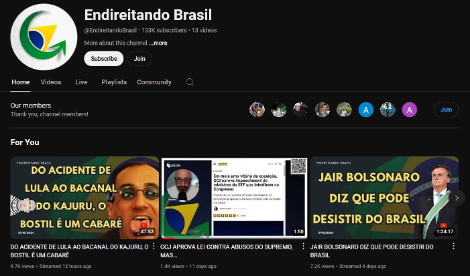
\includegraphics[width=\linewidth]{Imagens/Fig11.png}
\caption{Página principal do canal de Youtube \emph{Endireitando Brasil}.}
\label{fig-11}
\source{\textcite{endireitando2024youtube}.}
\end{minipage}
%\end{figure}
\hfill
% Segunda imagem
%\begin{figure}
\centering
\begin{minipage}[t]{0.45\textwidth}
\centering        

\includegraphics[width=\linewidth]{Imagens/Fig12.png}
\caption{Descrição do canal de Youtube \emph{Endireitando Brasil}.}
\label{fig-12}
\source{\textcite{endireitando2024youtube}.}
\end{minipage}
\end{figure}
    

\section{Postagens mais recorrentes por canal}\label{sec-postagens_recorrentes}

\subsection{O INFORMANTE}

%--- CÓDIGO DAS FIGURAS 13, 14, 15, 16, 17 ---%
\begin{figure}[h!]
    \centering
    % Primeira linha (2 figuras)
    \begin{minipage}[t]{0.31\textwidth}
        \centering
        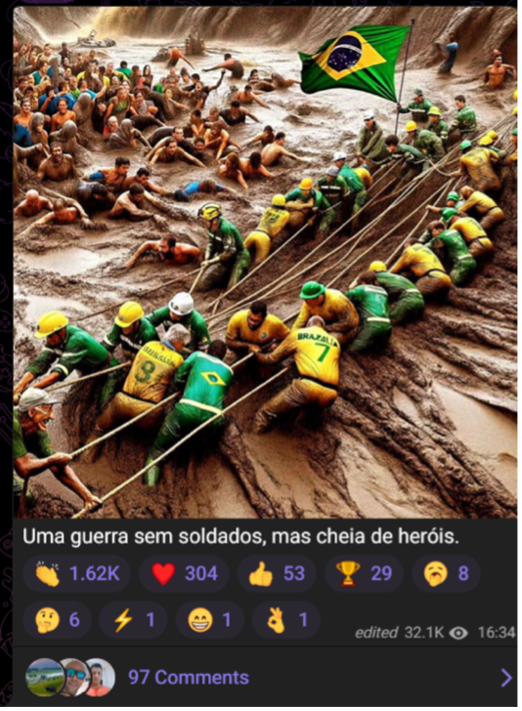
\includegraphics[width=\linewidth]{Imagens/Fig38.png}
        \caption{Postagem 1 do canal \emph{O Informante}.}
        \label{fig-13}
    \end{minipage}
    \hfill
    \begin{minipage}[t]{0.38\textwidth}
        \centering
        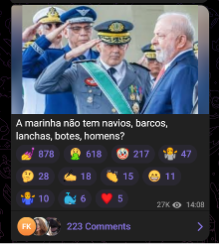
\includegraphics[width=\linewidth]{Imagens/Fig14.png}
        \caption{Postagem 2 do canal \emph{O Informante}.}
        \label{fig-14}
    \end{minipage}
    
    \vspace{0.2cm} % espaço entre linhas
    
    % Segunda linha (2 figuras)
    \begin{minipage}[t]{0.57\textwidth}
        \centering
        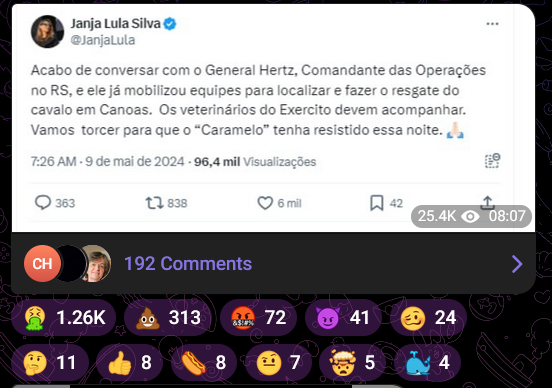
\includegraphics[width=\linewidth]{Imagens/Fig15_1.png}
        \caption{Postagem 3 do canal \emph{O Informante}.}
        \label{fig-15}
    \end{minipage}
    \hfill
    \begin{minipage}[t]{0.27\textwidth}
        \centering
        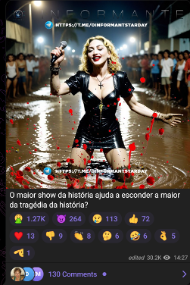
\includegraphics[width=\linewidth]{Imagens/Fig16.png}
        \caption{Postagem 4 do canal \emph{O Informante}.}
        \label{fig-16}
    \end{minipage}
    
    \vspace{0.2cm} % espaço entre linhas
    
    % Terceira linha (1 figura centralizada)
    \begin{minipage}[t]{0.39\textwidth}
        \centering
        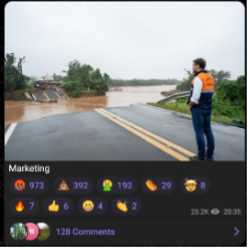
\includegraphics[width=\linewidth]{Imagens/Fig17.png}
        \caption{Postagem 5 do canal \emph{O Informante}.}
        \label{fig-17}
    \end{minipage}
    
    \source{\textcite{telegram2024}.}
\end{figure}



A primeira postagem (\Cref{fig-13}) tem 32,1 mil visualizações, 97 comentários e 2.023 reações, sendo as duas mais frequentes os emojis ``{\Symbola 👏}'' (``mãos aplaudindo'', demonstra aprovação) e ``{\Symbola ❤️}'' (``coração vermelho'', demonstra amor ou afeto). Nela, o enunciador \emph{O Informante} apresenta a imagem gerada por inteligência artificial de um grupo de homens em vestes verde e amarelo resgatando vítimas das enchentes, sendo que um deles está com a bandeira do Brasil hasteada. No cenário, a lama e a água se confundem. Abaixo da imagem, está a legenda: ``Uma guerra sem soldados, mas cheia de heróis''.

A segunda postagem (\Cref{fig-14}) tem 27 mil visualizações, 223 comentários e 1853 reações, sendo as duas mais frequentes os emojis ``{\Symbola 🤮}'' (``rosto vomitando'', demonstra nojo ou repulsa extrema) e ``{\Symbola 💅}'' (``esmalte de unha'', que pode demonstrar ironia, indiferença ou feminilidade). Nela, o enunciador \emph{O Informante} apresenta a imagem dos comandantes da Marinha, da Aeronáutica e do Exército, respectivamente, Marcos Sampaio Olsen, Marcelo Kanitz Damasceno e Tomás Miguel Ribeiro Paiva, da esquerda para a direita, prestando continência ao presidente Luiz Inácio Lula da Silva. A imagem é de Ricardo Stuckert, fotógrafo da Presidência da República. Abaixo da foto, está a legenda: ``A marinha não tem navios, barcos, lanchas, botes, homens?''.

A terceira postagem (\Cref{fig-15}) tem 25,4 mil visualizações, 192 comentários e 1753 reações, sendo as duas mais frequentes os emojis ``{\Symbola 🤮}'' (``rosto vomitando'') e ``{\Symbola 💩}'' (``cocô'', demonstra desprezo). Nela, o enunciador \emph{O Informante} apresenta uma captura de tela de uma postagem da primeira-dama Rosângela ``Janja'' Lula da Silva na plataforma X/Twitter. A imagem não acompanha a legenda. A primeira-dama declara:

\begin{quote}
    Acabo de conversar com o General Hertz, Comandante das Operações no RS, e ele já mobilizou equipes para localizar e fazer o resgate do cavalo em Canoas. Os veterinários do Exercito (sic) devem acompanhar. Vamos torcer para que o ``Caramelo'' tenha resistido essa noite. {\Symbola 🙏}
\end{quote}

A quarta postagem (\Cref{fig-16}) tem 30,2 mil visualizações, 130 comentários e 1767 reações, sendo as duas mais frequentes os emojis ``{\Symbola 🤮}'' (``rosto vomitando'') e ``{\Symbola 😈}'' (``rosto sorridente com chifres'', retrata a maldade e a figura cristã do diabo). Nela, o enunciador \emph{O Informante} apresenta a imagem gerada por inteligência artificial da cantora Madonna, em primeiro plano, com um microfone nas mãos, mergulhada até os joelhos em uma gigante poça de lama. Um efeito de respingo de sangue envolve a figura da artista. Em segundo plano, várias figuras humanas a observam. A peça gráfica contém o nome, o logotipo e o link do próprio canal \emph{O Informante}. Abaixo da imagem, está a legenda: ``O maior show da história ajuda a esconder a maior tragédia da história?''.

A quinta postagem (\Cref{fig-17}) tem 3,7 mil visualizações, 26 comentários e 202 reações, sendo as duas mais frequentes os emojis ``{\Symbola 🤬}'' (``rosto com símbolos na boca'', representa xingamentos e indignação) e ``{\Symbola 💩}'' (``cocô''). Nela, o enunciador \emph{O Informante} apresenta a imagem do Governador do Rio Grande do Sul, Eduardo Leite, contemplando parte de uma rodovia destruída durante o período das enchentes. Abaixo da imagem, está a legenda: ``Marketing''.

\subsection{MBL -- Movimento Brasil Livre}

%--- CÓDIGO DAS FIGURAS 18, 19, 20, 21, 22 ---%
\begin{figure}[h!]
    \centering
    % Primeira linha (3 figuras)
    \begin{minipage}[t]{0.3\textwidth}
        \centering
        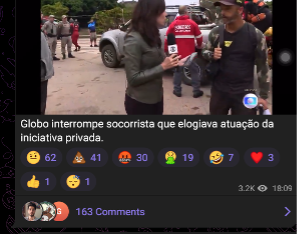
\includegraphics[width=\linewidth]{Imagens/Fig18.png}
        \caption{Postagem 1 do canal \emph{MBL -- Movimento Brasil Livre}.}
        \label{fig-18}
    \end{minipage}
    \hfill
    \begin{minipage}[t]{0.3\textwidth}
        \centering
        
\includegraphics[width=\linewidth]{Imagens/Fig19.png}
        \caption{Postagem 2 do canal \emph{MBL -- Movimento Brasil Livre}.}
        \label{fig-19}
    \end{minipage}
    \hfill
    \begin{minipage}[t]{0.3\textwidth}
        \centering
        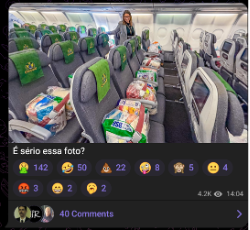
\includegraphics[width=\linewidth]{Imagens/Fig20.png}
        \caption{Postagem 3 do canal \emph{MBL -- Movimento Brasil Livre}.}
        \label{fig-20}
    \end{minipage}

    \vspace{0.5cm} % espaço entre as linhas de figuras

    % Segunda linha (2 figuras)
    \begin{minipage}[t]{0.40\textwidth}
        \centering
        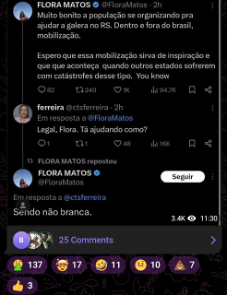
\includegraphics[width=\linewidth]{Imagens/Fig21.png}
        \caption{Postagem 4 do canal \emph{MBL -- Movimento Brasil Livre}.}
        \label{fig-21}
    \end{minipage}
    \hfill
    \begin{minipage}[t]{0.34\textwidth}
        \centering
        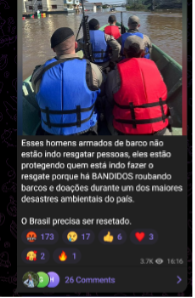
\includegraphics[width=\linewidth]{Imagens/Fig22.png}
        \caption{Postagem 5 do canal \emph{MBL -- Movimento Brasil Livre}.}
        \label{fig-22}
    \end{minipage}
    \source{\textcite{telegram2024}.}
\end{figure}

A primeira postagem (\Cref{fig-18}) tem 3,2 mil visualizações, 163 comentários e 164 reações, sendo as duas mais frequentes os emojis ``{\Symbola 🤨}'' (``rosto com sobrancelha levantada'', demonstra desconfiança, ceticismo e rejeição) e ``{\Symbola 💩}'' (``cocô''). Nela, o enunciador \emph{MBL -- Movimento Brasil Livre} apresenta a imagem de uma repórter entrevistando um homem em trajes de socorrista em um cenário enlameado. No canto inferior direito da imagem, observa-se o logo da Rede Globo e a inserção gráfica ``Ao Vivo'', que denota a transmissão em tempo real. Abaixo da imagem, está a legenda: ``Globo interrompe socorrista que elogiava atuação da iniciativa privada''.

A segunda postagem (\Cref{fig-19}) tem 4,8 mil visualizações, 38 comentários e 255 reações, sendo as duas mais frequentes os emojis ``{\Symbola 💩}'' (``cocô'') e ``{\Symbola 🤮}'' (``rosto vomitando''). Nela, o enunciador \emph{MBL -- Movimento Brasil Livre} apresenta a imagem da primeira-dama Janja, em primeiro plano, frente a um helicóptero sendo esvaziado com doações para as vítimas da catástrofe, em segundo plano. Abaixo da imagem, está a legenda: ``Blogueirinha tá curtindo''.

A terceira postagem (\Cref{fig-20}) tem 4,2 mil visualizações, 40 comentários e 238 reações, sendo as duas mais frequentes os emojis ``{\Symbola 🤮}'' (``rosto vomitando'') e ``{\Symbola 🤣}'' (``rolando no chão de rir'', demonstra riso histérico). Nela, o enunciador \emph{MBL -- Movimento Brasil Livre} apresenta a imagem da primeira-dama Janja sozinha em um avião em que, em vez de de passageiros, cada cadeira é ocupada por uma cesta básica destinada às vítimas da catástrofe. Abaixo da imagem, está a legenda: ``É sério essa foto?''.

A quarta postagem (\Cref{fig-21}) tem 3,4 mil visualizações, 25 comentários e 260 reações, sendo as duas mais frequentes os emojis ``{\Symbola 🤮}'' (``rosto vomitando'') e ``{\Symbola 🤯}'' (``cabeça explodindo'', demonstra choque ou espanto). Nela, o enunciador \emph{MBL -- Movimento Brasil Livre} apresenta uma captura de tela de um diálogo em três postagens da plataforma X/Twitter. A primeira postagem é da usuária ``FLORA MATOS'':

\begin{quote}
    Muito bonito a população se organizando para ajudar a galera no RS. Dentro e fora do brasil (sic), mobilização. Espero que essa mobilização sirva de inspiração e que que (sic) aconteça quando outros estados sofrerem com catástrofes desse tipo. You know
\end{quote}
A usuária ``ferreira'' responde: ``Legal, Flora, Tá ajudando como?''. Por fim, ``FLORA MATOS'' replica: ``Sendo não branca''. A imagem não acompanha legenda.

A quinta postagem (\Cref{fig-22}) tem 3,7 mil visualizações, 26 comentários e 202 reações, sendo as duas mais frequentes os emojis ``{\Symbola 🤬}'' (``rosto com símbolos na boca'') e ``{\Symbola 😢}'' (``rosto chorando'', demonstra tristeza e dor). Nela, o enunciador \emph{MBL -- Movimento Brasil Livre} apresenta a imagem de cinco homens armados e vestidos em coletes salva-vidas. Os cinco assentam-se em um barco que navega pela área alagada de uma cidade. Abaixo da imagem, está a legenda:

\begin{quote}
    Esses homens armados de barco não estão indo resgatar pessoas, eles estão protegendo quem está indo fazer o resgate porque há BANDIDOS roubando barcos e doações durante um dos maiores desastres ambientais do país. O Brasil precisa ser resetado.
\end{quote}

\subsection{Paladin}

%--- CÓDIGO DAS FIGURAS 23, 24, 25, 26, 27 ---%
\begin{figure}[h!]
    \centering
    % Primeira linha (2 figuras)
    \begin{minipage}[t]{0.50\textwidth}
        \centering
        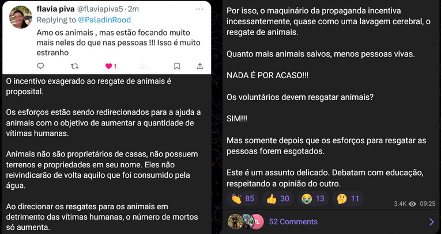
\includegraphics[width=\linewidth]{Imagens/Fig23.png}
        \caption{Postagem 1 do canal \emph{Paladin}.}
        \label{fig-23}
    \end{minipage}
    \hfill
    \begin{minipage}[t]{0.46\textwidth}
        \centering
        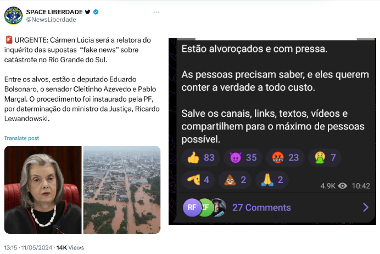
\includegraphics[width=\linewidth]{Imagens/Fig24.png}
        \caption{Postagem 2 do canal \emph{Paladin}.}
        \label{fig-24}
    \end{minipage}
    
    \vspace{0.2cm} % espaço entre linhas
    
    % Segunda linha (2 figuras)
    \begin{minipage}[t]{0.50\textwidth}
        \centering
        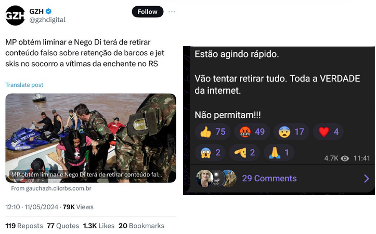
\includegraphics[width=\linewidth]{Imagens/Fig25.png}
        \caption{Postagem 3 do canal \emph{Paladin}.}
        \label{fig-25}
    \end{minipage}
    \hfill
    \begin{minipage}[t]{0.46\textwidth}
        \centering
        
\includegraphics[width=\linewidth]{Imagens/Fig26.png}
        \caption{Postagem 4 do canal \emph{Paladin}.}
        \label{fig-26}
    \end{minipage}
    
    \vspace{0.2cm} % espaço entre linhas
    
    % Terceira linha (1 figura centralizada)
    \begin{minipage}[t]{0.50\textwidth}
        \centering
        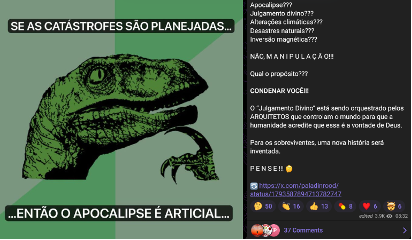
\includegraphics[width=\linewidth]{Imagens/Fig27.png}
        \caption{Postagem 5 do canal \emph{Paladin}.}
        \label{fig-27}
    \end{minipage}
    
    \source{\textcite{telegram2024}.}
\end{figure}

A primeira postagem (\Cref{fig-23}) tem 3,4 mil visualizações, 52 comentários e 139 reações, sendo as duas mais frequentes os emojis ``{\Symbola 👏}'' (``mãos aplaudindo'') e ``{\Symbola 👍}'' (``polegar para cima'', demonstra aprovação). Nela, o enunciador \emph{Paladin} apresenta uma captura de tela de uma postagem na plataforma X/Twitter da usuária ``flavia piva'': ``Amo os animais, mas estão focando muito mais neles do que nas pessoas !!! Isso é muito estranho''. Abaixo da imagem, está a legenda:

\begin{quote}
    O incentivo exagerado ao resgate de animais é proposital. Os esforços estão sendo redirecionados para a ajuda a animais com o objetivo de aumentar a quantidade de vítimas humanas. Animais não são proprietários de casas, não possuem terrenos e propriedades em seu nome. Eles não reivindicarão de volta aquilo que foi consumido pela água. Ao direcionar os resgates para os animais em detrimento das vítimas humanas, o número de mortos só aumenta. Por isso, o maquinário da propaganda incentiva incessantemente, quase como uma lavagem cerebral, o resgate de animais. Quanto mais animais salvos, menos pessoas vivas. NADA É POR ACASO!!! Os voluntários devem resgatar animais? SIM!!! Mas somente depois que os esforços para resgatar as pessoas forem esgotados. Este é um assunto delicado. Debatam com educação, respeitando a opinião do outro.
\end{quote}

A segunda postagem (\Cref{fig-24}) tem 4,9 mil visualizações, 27 comentários e 156 reações, sendo as duas mais frequentes os emojis ``{\Symbola 👍}'' (``polegar para cima'') e ``{\Symbola 😈}'' (``rosto sorridente com chifres''). Nela, o enunciador \emph{Paladin} apresenta uma captura de tela de uma postagem na plataforma X/Twitter do usuário ``SPACE LIBERDADE'':

\begin{quote}
URGENTE: Cármen Lúcia será a relatora do inquérito das supostas ``fake news'' sobre catástrofe no Rio Grande do Sul. Entre os alvos, estão o deputado Eduardo Bolsonaro, o senador Cleitinho Azevedo e Pablo Marçal. O procedimento foi instaurado pela PF, por determinação do ministro da Justiça, Ricardo Lewandowski.
\end{quote}
Abaixo da imagem, está a legenda: ``Estão alvoroçados e com pressa. As pessoas precisam saber, e eles querem conter a verdade a todo custo. Salve os canais, links, textos, vídeos e compartilhem para o máximo de pessoas possível''.

A terceira postagem (\Cref{fig-25}) tem 4,7 mil visualizações, 29 comentários e 150 reações, sendo as duas mais frequentes os emojis ``{\Symbola 👍} (``polegar para cima'') e ``{\Symbola 🤬}'' (``rosto com símbolos na boca''). Nela, o enunciador \emph{Paladin} apresenta uma captura de tela de uma postagem na plataforma X/Twitter do usuário ``GZH'': ``MP obtém liminar e Nego Di terá de retirar conteúdo falso sobre retenção de barcos e jet skis no socorro a vítimas da enchente no RS''. Abaixo da imagem, está a legenda: ``Estão agindo rápido. Vão tentar retirar tudo. Toda a VERDADE da internet. Não permitam!!!''.

A quarta postagem (\Cref{fig-26}) tem 15,9 mil visualizações, 24 comentários e 114 reações, sendo as duas mais frequentes os emojis ``{\Symbola 🤯}'' (``cabeça explodindo'') e ``{\Symbola 🤬}'' (``rosto com símbolos na boca''). Nela, o enunciador \emph{Paladin} apresenta uma peça gráfica imitando uma folha de papel antiga. A parte central superior da imagem abriga a expressão ``TOP SECRET'', que significa altamente secreto. No papel, em formato de lista, está escrito:

\begin{quote}
Plano Marshall Rio Grande do Sul: Desapropriação; restrições severas de uso da terra; zonas de exclusão; lockdown climático; realocação em massa; monitoramento massivo da população.
\end{quote}

Abaixo da imagem, está a legenda: ``Rio Grande do Sul: O Plano Marshall do Brasil visa implementar imediatamente''.

A quinta postagem (\Cref{fig-27}) tem 3,9 mil visualizações, 37 comentários e 99 reações, sendo as duas mais frequentes os emojis ``{\Symbola 🤔}'' (``rosto pensativo'', demonstra contemplação de algo ou um pensamento profundo) e ``{\Symbola 👏}'' (``mãos aplaudindo''). Nela, o enunciador \emph{Paladin} apresenta uma peça gráfica em formato de meme. Um dinossauro verde em posição pensativa contempla as palavras: ``Se as catástrofes são planejadas... então o apocalipse é articial [sic]''. Abaixo da imagem, está a legenda: 

\begin{quote}
Apocalipse??? Julgamento divino??? Alterações climáticas??? Desastres naturais??? Inversão magnética??? NÃO, M A N I P U L A Ç Ã O!!! Qual o propósito??? CONDENAR VOCÊ!!! O ``Julgamento Divino'' está sendo orquestrado pelos ARQUITETOS que controlam o mundo para que a humanidade acredite que essa é a vontade de Deus. Para os sobreviventes, uma nova história será inventada. P E N S E !!! {\Symbola 🤔}
\end{quote}

\subsection{DIREITA BRASIL}
%--- CÓDIGO DAS FIGURAS 28, 29, 30, 31, 32 ---%
\begin{figure}[h!]
    \centering
    % Primeira linha (3 figuras)
    \begin{minipage}[t]{0.30\textwidth}
        \centering
        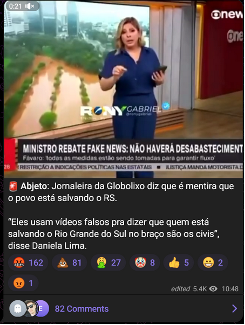
\includegraphics[width=\linewidth]{Imagens/Fig28.png}
        \caption{Postagem 1 do canal \emph{DIREITA BRASIL}.}
        \label{fig-28}
    \end{minipage}\hfill
    \begin{minipage}[t]{0.21\textwidth}
        \centering
        
\includegraphics[width=\linewidth]{Imagens/Fig29.png}
        \caption{Postagem 2 do canal \emph{DIREITA BRASIL}.}
        \label{fig-29}
    \end{minipage}\hfill
    \begin{minipage}[t]{0.32\textwidth}
        \centering
        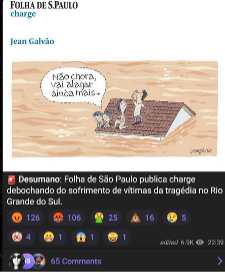
\includegraphics[width=\linewidth]{Imagens/Fig30.png}
        \caption{Postagem 3 do canal \emph{DIREITA BRASIL}.}
        \label{fig-30}
    \end{minipage}

    \vspace{0.3cm} % espaço entre as linhas

    % Segunda linha (2 figuras)
    \begin{minipage}[t]{0.47\textwidth}
        \centering
        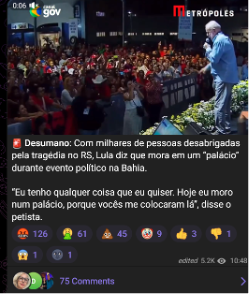
\includegraphics[width=\linewidth]{Imagens/Fig31.png}
        \caption{Postagem 4 do canal \emph{DIREITA BRASIL}.}
        \label{fig-31}
    \end{minipage}\hfill
    \begin{minipage}[t]{0.29\textwidth}
        \centering
        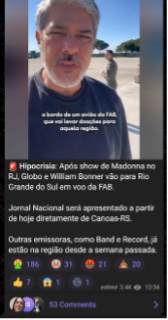
\includegraphics[width=\linewidth]{Imagens/Fig32.png}
        \caption{Postagem 5 do canal \emph{DIREITA BRASIL}.}
        \label{fig-32}
    \end{minipage}
    
    \source{\textcite{telegram2024}.}
\end{figure}

A primeira postagem (\Cref{fig-28}) tem 5,4 mil visualizações, 82 comentários e 286 reações, sendo as duas mais frequentes os emojis ``{\Symbola 🤬}'' (``rosto com símbolos na boca'') e ``{\Symbola 💩}'' (``cocô''). Nela, o enunciador \emph{DIREITA BRASIL} apresenta a imagem de, em primeiro plano, a repórter Daniela Lima apresentando um programa jornalístico da Globo News, \emph{Edição das 18}. Em segundo plano, atrás da repórter, há uma transmissão em uma tela das enchentes do Rio Grande do Sul. No canto superior direito da imagem, observa-se o logo do canal Globo News. Abaixo da imagem, está a legenda: ``Abjeto: Jornaleira da Globolixo diz que é mentira que o povo está salvando o RS. `Eles usam vídeos falsos pra dizer que quem está salvando o Rio Grande do Sul no braço são os civis', disse Daniela Lima''.

A segunda postagem (\Cref{fig-29}) tem 3,9 mil visualizações, 85 comentários e 281 reações, sendo as duas mais frequentes os emojis ``{\Symbola 💩}'' (``cocô'') e ``{\Symbola 🤡}'' (``rosto de palhaço'', indica que algo ou alguém é tolo ou idiota). Nela, o enunciador \emph{DIREITA BRASIL} apresenta a imagem de uma influenciadora digital conversando com a câmera. Abaixo da imagem, está a legenda: ``Se Lascou: Influenciadora petista que fez piada da tragédia no RS publica vídeo chorando e se vitimizando após ter conta no TikTok derrubada''.

A terceira postagem (\Cref{fig-30}) tem 6,9 mil visualizações, 65 comentários e 285 reações, sendo as duas mais frequentes os emojis ``{\Symbola 😡}'' (``rosto furioso'', demonstra raiva ou irritação intensa) e ``{\Symbola 🤬}'' (``rosto com símbolos na boca''). Nela, o enunciador \emph{DIREITA BRASIL} apresenta uma charge da Folha de S. Paulo sobre as enchentes do Rio Grande do Sul. A charge retrata uma família no topo do telhado de uma casa rodeada por água. Uma das crianças diz à outra: ``Não chora, vai alagar ainda mais...''. Abaixo da imagem, está a legenda: ``Desumano: Folha de São Paulo (sic) publica charge debochando do sofrimento de vítimas da tragédia no Rio Grande do Sul''.

A quarta postagem (\Cref{fig-31}) tem 5,2 mil visualizações, 75 comentários e 247 reações, sendo as duas mais frequentes os emojis ``{\Symbola 🤬}'' (``rosto com símbolos na boca'') e ``{\Symbola 🤮}'' (``rosto vomitando''). Nela, o enunciador \emph{DIREITA BRASIL} apresenta a imagem do presidente Lula no topo de um palco conversando com um público trajando vermelho à sua frente. Abaixo da imagem, está a legenda:

\begin{quote}
    Desumano: Com milhares de pessoas desabrigadas pela tragédia no RS, Lula diz que mora em um ``palácio'' durante evento político na Bahia. ``Eu tenho qualquer coisa que eu quiser. Hoje eu moro num palácio, porque vocês me colocaram lá'', disse o petista.
\end{quote}

A quinta postagem (\Cref{fig-32}) tem 3,4 mil visualizações, 53 comentários e 267 reações, sendo as duas mais frequentes os emojis ``{\Symbola 🤮}''' (``rosto vomitando'') e ``{\Symbola 🤡}'' (``rosto de palhaço''). Nela, o enunciador \emph{DIREITA BRASIL} apresenta uma captura de tela de um vídeo do repórter William Bonner falando em frente a uma câmera. A imagem começa a legendar sua fala: ``A bordo de um avião da FAB, que vai levar doações para aquela região''. Abaixo da imagem, está a legenda:

\begin{quote}
    Hipocrisia: Após show de Madonna no RJ, Globo e William Bonner vão para Rio Grande do Sul em voo da FAB. Jornal Nacional será apresentado a partir de hoje diretamente de Canoas-RS. Outras emissoras, como Band e Record, já estão na região desde a semana passada.
\end{quote}

\subsection{SALDANHA -- Endireitando Brasil}
%--- CÓDIGO DAS FIGURAS 33, 34, 35, 36, 37 ---%
\begin{figure}[h!]
    \centering
    % Primeira linha (3 figuras)
    \begin{minipage}[t]{0.3\textwidth}
        \centering
        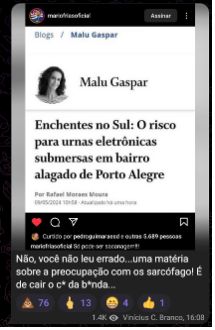
\includegraphics[width=\linewidth]{Imagens/Fig33.png}
        \caption{Postagem 1 do canal \emph{SALDANHA -- Endireitando Brasil}.}
        \label{fig-33}
    \end{minipage}
    \hfill
    \begin{minipage}[t]{0.3\textwidth}
        \centering
        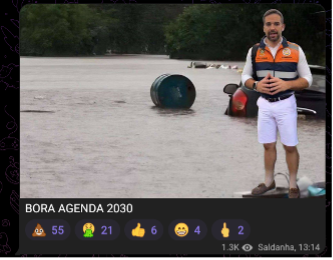
\includegraphics[width=\linewidth]{Imagens/Fig34.png}
        \caption{Postagem 2 do canal \emph{SALDANHA -- Endireitando Brasil}.}
        \label{fig-34}
    \end{minipage}
    \hfill
    \begin{minipage}[t]{0.3\textwidth}
        \centering
        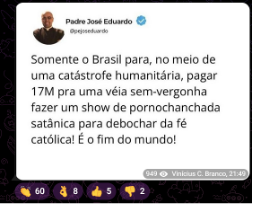
\includegraphics[width=\linewidth]{Imagens/Fig35.png}
        \caption{Postagem 3 do canal \emph{SALDANHA -- Endireitando Brasil}.}
        \label{fig-35}
    \end{minipage}

    \vspace{0.5cm} % espaço entre as linhas de figuras

    % Segunda linha (2 figuras)
    \begin{minipage}[t]{0.25\textwidth}
        \centering
        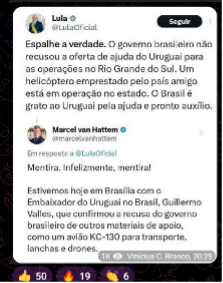
\includegraphics[width=\linewidth]{Imagens/Fig36.png}
        \caption{Postagem 4 do canal \emph{SALDANHA -- Endireitando Brasil}.}
        \label{fig-36}
    \end{minipage}
    \hfill
    \begin{minipage}[t]{0.35\textwidth}
        \centering
        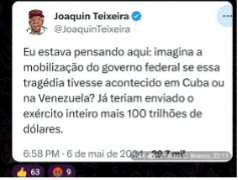
\includegraphics[width=\linewidth]{Imagens/Fig37.png}
        \caption{Postagem 5 do canal \emph{SALDANHA -- Endireitando Brasil}.}
        \label{fig-37}
    \end{minipage}
    \source{\textcite{telegram2024}.}
\end{figure}

A primeira postagem (\Cref{fig-33}) tem 1,4 mil visualizações e 94 reações, sendo as duas mais frequentes os emojis ``{\Symbola 💩}'' (``cocô'') e ``{\Symbola 🖕}'' (``dedo do meio'', um gesto insultuoso). Nela, o enunciador \emph{SALDANHA -- Endireitando Brasil} apresenta uma captura de tela da manchete de uma reportagem \textit{online} de O Globo assinada pela jornalista Malu Gaspar sobre as enchentes do Rio Grande do Sul: ``Enchentes no Sul: O risco para urnas eletrônicas submersas em bairro alagado de Porto Alegre''. Abaixo da imagem, está a legenda: ``Não, você não leu errado... uma matéria sobre a preocupação com os sarcófago (sic)! É de cair o c* da b*nda...''. O enunciador usa do termo ``sarcófago'', ``cova coberta de terra, onde se sepultam os mortos'', para associar as urnas eletrônicas às urnas funerárias, ``pequeno recipiente, [...] utilizado para depositar as cinzas dos defuntos cremados'' \cite{michaelis2024}. Atribui às urnas eletrônicas e, como consequência, ao sistema eleitoral brasileiro, a velhice e a obsolescência.

A segunda postagem (\Cref{fig-34}) tem 1,3 mil visualizações e 88 reações, sendo as duas mais frequentes os emojis ``{\Symbola 💩}'' (``cocô'') e ``{\Symbola 🤮}'' (``rosto vomitando''). Nela, o enunciador \emph{SALDANHA -- Endireitando Brasil} apresenta uma montagem da figura do Governador do Rio Grande do Sul Eduardo Leite sob uma fotografia dos alagamentos no estado. Abaixo da imagem, está a legenda: ``BORA AGENDA 2030''.

A terceira postagem (\Cref{fig-35}) tem 949 visualizações e 75 reações, sendo as duas mais frequentes os emojis ``{\Symbola 👏}'' (``mãos aplaudindo'') e ``{\Symbola 👌}'' (``sinal de ok'', demonstra aprovação). Nela, o enunciador \emph{SALDANHA -- Endireitando Brasil} apresenta uma captura de tela de uma postagem na plataforma X/Twitter do usuário ``Padre José Eduardo'': ``Somente o Brasil para, no meio de uma catástrofe humanitária, pagar 17M pra uma véia [sic] sem-vergonha fazer um show de pornochanchada satânica para debochar da fé católica! É o fim do mundo!''. A imagem não acompanha legenda.

A quarta postagem (\Cref{fig-36}) tem mil visualizações e 75 reações, sendo as duas mais frequentes os emojis ``{\Symbola 👍}'' (``polegar para cima'') e ``{\Symbola 🔥}'' (``fogo'', demonstra ardor e entusiasmo). Nela, o enunciador \emph{SALDANHA -- Endireitando Brasil} apresenta uma captura de tela de um diálogo em duas postagens da plataforma X/Twitter. A primeira postagem é do Presidente Lula: 

\begin{quote}
    Espalhe a verdade. O governo brasileiro não recusou a oferta de ajuda do Uruguai para as operações no Rio Grande do Sul. Um helicóptero emprestado pelo país amigo está em operação no estado. O Brasil é grato ao Uruguai pela ajuda e pronto auxílio.
\end{quote}

O usuário ``Marcel van Hattem'' responde:
\begin{quote}
    Mentira. Infelizmente, mentira! Estivemos hoje em Brasília com o Embaixador do Uruguai no Brasil, Guillermo Valles, que confirmou a recusa do governo brasileiro de outros materiais de apoio, como um avião KC-130 para transporte, lanchas e drones.
\end{quote}
A imagem não acompanha legenda.

A quinta postagem (\Cref{fig-37}) tem 1,4 mil visualizações e 72 reações, sendo as duas mais frequentes os emojis  ``{\Symbola 👍}'' (``polegar para cima'') e ``{\Symbola 🤬}'' (``rosto com símbolos na boca''). Nela, o enunciador \emph{SALDANHA -- Endireitando Brasil} apresenta uma captura de tela de uma postagem na plataforma X/Twitter do usuário ``Joaquin Teixeira'': ``Eu estava pensando aqui: imagina a mobilização do governo federal se essa tragédia tivesse acontecido em Cuba ou na Venezuela? Já teriam enviado o exército inteiro mais 100 trilhões de dólares''. A imagem não acompanha legenda.

\section{Tipologias discursivas do ecossistema desinformacional}\label{sec-tipologias-discur}
Juntamente com os textos e discursos desinformacionais, outros fenômenos emergem e se entrelaçam, compondo um verdadeiro cipoal que desafia a compreensão linear e exige uma abordagem multifacetada para serem compreendidos.  Esse emaranhado de fenômenos, em que dificilmente a desinformação (entendida como conteúdo enganoso/mentiroso) se apresenta de forma pura, é chamado por \textcite{alzamora2021} de \emph{ecossistema desinformacional} que se baseia numa dinâmica transmídia. Assim, propomos, de forma preliminar e dedutiva, as seguintes tipologias discursivas do ecossistema desinformacional\footnote{A tipologia aqui apresentada foi concebida a partir da análise de um corpus descrito no item \nameref{sec-metodologia}. Trata-se, portanto, de uma categorização provisória, formulada de maneira dedutiva, que poderá ser revista ou ampliada em trabalhos futuros.}:

\begin{itemize}
    \item Conteúdo enganoso; 
    \item Conteúdo declaratório; 
    \item Discurso de ódio; 
    \item Ironia; 
    \item Memes; 
    \item Teorias conspiratórias.
\end{itemize}

A seguir, serão apresentados exemplos de cada tipologia com base na referida pesquisa. Cabe dizer que uma mesma postagem pode ter elementos de uma ou mais tipologias. 

\subsection{Conteúdo enganoso}
O conteúdo enganoso pode ser definido como um conteúdo que parece verdadeiro, mas apresenta uma informação mentirosa.

%--- CÓDIGO DA FIGURA 38 ---%
\begin{figure}[ht]
    \centering
    % Primeira linha (3 figuras)
    \begin{minipage}{0.45\textwidth}
        \centering
        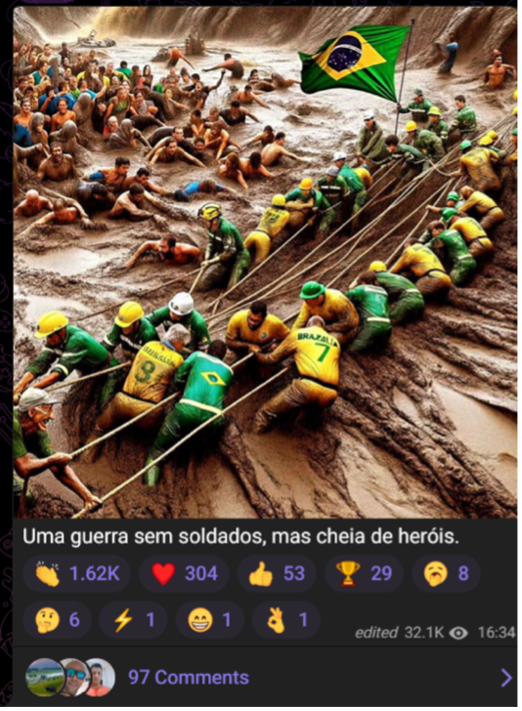
\includegraphics[width=\textwidth]{Imagens/Fig38.png}
        \caption{Conteúdo enganoso.}
        \label{fig-38}
        \source{\textcite{telegram2024}.}
    \end{minipage}
    \end{figure}

No caso em pauta (\Cref{fig-38}), civis vestidos de verde e amarelo tentam salvar pessoas das enchentes no RS. Discursos mentirosos de que civis e não os governos federal e estadual atuaram nas enchentes, foram amplamente encontrados na referida pesquisa. A imagem é facilmente reconhecível como sendo produto de inteligência artificial. 

\subsection{Conteúdo declaratório}
No caso do conteúdo declaratório, não existe necessariamente um conteúdo verdadeiro ou mentiroso. Trata-se de uma asserção baseada na opinião e, portanto, na crença de quem enuncia.

%--- CÓDIGO DA FIGURA 39 ---%
\begin{figure}[ht]
    \centering
    % Primeira linha (3 figuras)
    \begin{minipage}{.45\textwidth}
        \centering
        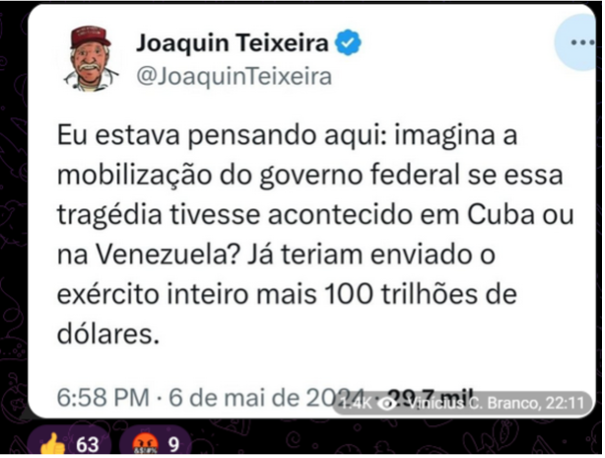
\includegraphics[width=\textwidth]{Imagens/Fig39.png}
        \caption{Conteúdo declaratório.}
        \label{fig-39}
        \source{\textcite{telegram2024}.}
    \end{minipage}
    \end{figure}
    
No caso em tela (\Cref{fig-39}), o usuário @JoaquinTeixeira acredita que se as enchentes tivessem ocorrido na Venezuela, o governo federal, por ser um governo de esquerda, teria se empenhado muito mais do que o fez, segundo ele, em relação à catástrofe climática do RS. 

\subsection{Ironia}
Já a ironia diz respeito a uma estratégia enunciativa em que se diz algo no enunciado, mas se nega esse dito pela enunciação. Para Fiorin,

\begin{quote}
    A ironia apresenta uma atitude do enunciador, pois é utilizada para criar sentidos que vão do gracejo até o sarcasmo, passando pelo escárnio, pela zombaria, pelo desprezo, etc. Na verdade, são duas vozes em conflito, uma expressando o inverso do que disse a outra \cite[p. 70]{fiorin2014}.
\end{quote}

%--- CÓDIGO DA FIGURA 40 ---%
\begin{figure}[ht]
    \centering
    \begin{minipage}{.40\textwidth}
        \centering
        
\includegraphics[width=\textwidth]{Imagens/Fig40.png}
        \caption{Ironia.}
        \label{fig-40}
        \source{\textcite{telegram2024}.}
    \end{minipage}
    \end{figure}
    
No caso em questão (\Cref{fig-40}), compreende-se que o enunciador da postagem ao chamar a primeira-dama de \emph{blogueirinha}, ironiza a presença dela nas enchentes do Rio Grande do Sul uma vez que não estaria ali para ajudar, mas para aparecer (assim como os blogueiros). 

\subsection{Discurso de ódio}
Acerca do discurso de ódio, inúmeros trabalhos têm se debruçado sobre o tema. Como não se trata do tema central deste trabalho, adotaremos a definição de \textcite{brugger2007}, que nos parece suficiente para definir o fenômeno: 

\begin{quote}
    O discurso do ódio refere-se a palavras que tendem a insultar, intimidar ou assediar pessoas em virtude de sua raça, cor, etnicidade, nacionalidade, sexo ou religião, ou que têm a capacidade de instigar violência, ódio ou discriminação contra tais pessoas \cite[p.118]{brugger2007}.
\end{quote}

%--- CÓDIGO DA FIGURA 41 ---%
\begin{figure}[ht]
    \centering
    \begin{minipage}{0.75\textwidth}
        \centering
        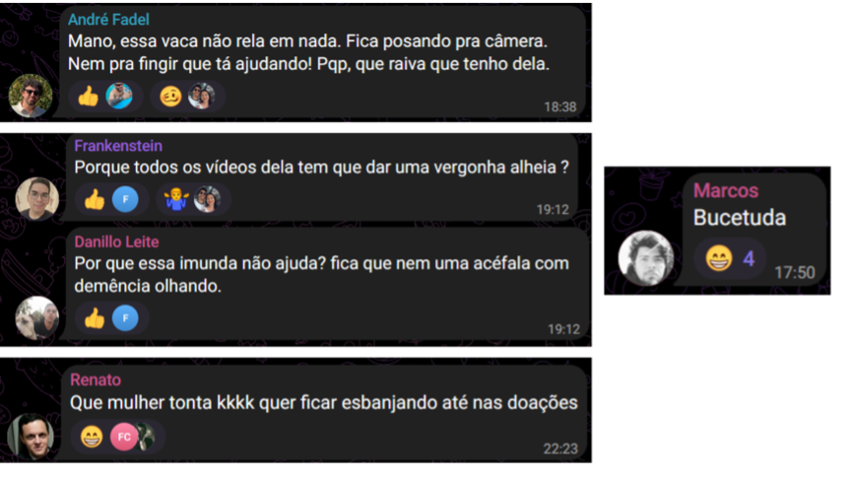
\includegraphics[width=\textwidth]{Imagens/Fig41.png}
        \caption{Discurso de ódio. Optou-se por desidentificar os autores dos comentários, uma vez que veiculam discurso de ódio. Embora esta figura não integre as 25 postagens selecionadas para o corpus, ela se refere a comentários feitos à postagem apresentada na \Cref{fig-40}. Sua inclusão tem como objetivo evidenciar que, nos comentários, o discurso de ódio se manifesta com maior veemência e intensidade.}
        \label{fig-41}
        \source{\textcite{telegram2024}.}
    \end{minipage}
    \end{figure}
    
O exemplo trazido (\Cref{fig-41}) refere-se a comentários injuriosos e xingamentos feitos à primeira-dama Janja no contexto das enchentes do RS. 

Além disso, o discurso de ódio nas postagens analisadas se materializa a partir das reações em emoji: os emojis ``{\Symbola 💩}'' (``cocô'') e ``{\Symbola 🤮}'' (``rosto vomitando'') são associados à primeira-dama Janja (\Cref{fig-19,fig-20}) em demonstrações de desprezo extremo de teor misógino; o emoji ``{\Symbola 💅}'' (``esmalte de unha''), associa uma crítica irônica à suposta inoperância do presidente Lula e dos comandantes do exército (\Cref{fig-14}) e se relaciona com uma lógica misógina e homofóbica para desqualificá-los.

\subsection{Memes}
Já os memes são mensagens que circulam no contexto da internet ``quase sempre de tom jocoso ou irônico que podem ou não ser acompanhadas por uma imagem ou vídeo e que é intensamente compartilhada por usuários nas mídias sociais'' \cite[p. 60]{torres2016}.

%--- CÓDIGO DA FIGURA 42 ---%
\begin{figure}[ht]
    \centering
    \begin{minipage}{.75\textwidth}
        \centering
        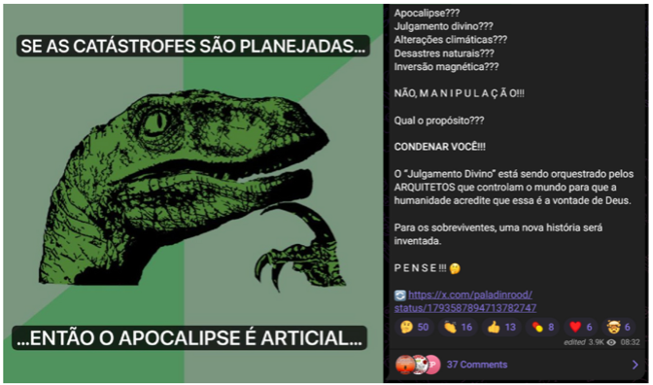
\includegraphics[width=\textwidth]{Imagens/Fig42.png}
        \caption{Memes.}
        \label{fig-42}
        \source{\textcite{telegram2024}.}
    \end{minipage}
    \end{figure}
    
O caso em pauta (\Cref{fig-42}) traz o meme Philosoraptor (ou dinossauro filósofo) surgido em 2008 \cite{museudosememes2025}. A imagem apresenta um dinossauro Velociraptor com uma expressão pensativa, como se estivesse profundamente refletindo sobre uma questão complexa ou paradoxal.

\subsection{Teorias conspiratórias}
Por fim, as teorias conspiratórias ``referem-se à criação de uma explicação `alternativa' ou `fantasiosa' para fatos que normalmente contrariam a versão oficial e politicamente correta de um determinado acontecimento'' \cite[p. 2]{rezende2019}. \textcite{aggio2021} acrescenta que:

\begin{quote}
    Nas palavras de um dos maiores estudiosos do assunto, Joseph Uscinsky (2020), teorias da conspiração se definem pela tentativa de explicação de um evento passado, presente ou futuro que elege como causa primária de sua ocorrência o envolvimento obscuro de um pequeno grupo de pessoas poderosas que atua em favor de seus interesses e contra o bem comum \cite[p. 67]{aggio2021}. 
\end{quote}

%--- CÓDIGO DA FIGURA 43 ---%
\begin{figure}[ht]
    \centering
    \begin{minipage}{.60\textwidth}
        \centering
        
\includegraphics[width=\textwidth]{Imagens/Fig26.png}
        \caption{Teorias conspiratórias.}
        \label{fig-43}
        \source{\textcite{telegram2024}.}
    \end{minipage}
    \end{figure}
    
No caso em pauta (\Cref{fig-43}) o enunciador da postagem diz estar em curso o chamado ``Plano Marshall Rio Grande do Sul'', em cujas medidas estariam a desapropriação de terras pelo governo federal após as enchentes, uma vez que o governo federal seria, de acordo com o enunciador e enunciatários da postagem, \emph{comunista}.

Cabe dizer, por fim, que uma mesma postagem pode ter elementos de uma ou mais tipologias. Além disso, embora pertençam a categorias distintas (como gêneros do discurso, figuras de linguagem e temas), as tipologias podem ser compreendidas a partir das modalidades do crer e do sentir, o que lhes conferem um estatuto semiótico. As tipologias associadas ao fazer-crer incluem o conteúdo enganoso, o conteúdo declaratório e as teorias conspiratórias. Já as associadas ao fazer-sentir são a ironia, o discurso de ódio e os memes. Enquanto as primeiras operam, \textit{a priori}, de forma fazer-crer o enunciatário, as últimas visam a afetá-lo sensivelmente. Do ponto de vista interacional, as tipologias voltadas ao fazer-crer se inscrevem no regime de manipulação, ao passo que aquelas voltadas ao fazer-sentir pertencem ao regime de ajustamento. Considerando-se, no entanto, que essas tipologias são categorias abstratas e podem coexistir em uma mesma textualidade, é plausível afirmar que, na prática, as modalidades do fazer-crer e do fazer-sentir não se manifestem de forma separada, mas sobreposta.

\section{Discursos (temas) mais recorrentes}\label{sec-discursos_rec}
No nível discursivo, as estruturas narrativas se são tematizadas e figurativizadas. Figuras são elementos com maior densidade sêmica e que remetem a elementos do mundo natural; já temas são abstratos, organizam e dão sentido às figuras \cite{greimas2008}. Assim, a partir da análise temática das 25 postagens coletadas sobre as enchentes ocorridas no Rio Grande do Sul durante o primeiro semestre de 2024, observaram-se as recorrências a seguir. 

Primeiramente, destacou-se o tema da ação dos civis, frequentemente figurativizada nas iniciativas de socorro e apoio às vítimas, em contraste com o tema da negligência do governo em atender de forma eficaz às demandas geradas pelo desastre. Essa negligência foi associada, em algumas postagens, à ideia de uma intenção deliberada do governo de permitir que civis morressem ou perdessem seus bens, o que leva ao próximo tema: a expropriação de terras.

O tema da expropriação de terras foi mencionado como parte de um suposto uso estratégico das enchentes pelo governo. Segundo essas postagens, a inação diante da catástrofe climática teria como objetivo forçar o deslocamento de comunidades e permitir a apropriação de suas terras e propriedades. Esse discurso também relaciona essa ação ao tema do comunismo, sugerindo que o governo utilizaria princípios associados a essa ideologia para justificar a expropriação, colocando-a como uma tentativa de redistribuição de terras ou controle econômico.

Outro tema identificado foi a ênfase no resgate de animais, apontada como uma estratégia para desviar a atenção da população. De acordo com o corpus analisado, o destaque dado ao salvamento de animais servia para ocultar o fato de que civis estavam morrendo. Esse tema também sugere que a prioridade dada aos animais em detrimento de seres humanos reforça uma hierarquia de valores que desumaniza as vítimas das enchentes. 

Por fim, emergiu o tema do comunismo, frequentemente ligado ao governo em discursos que sugerem teorias conspiratórias ou associações ideológicas, especialmente em postagens de caráter polarizado. Essa temática revela como as enchentes foram incorporadas a discursos mais amplos de crítica política e ideológica. 

Outro tema observado foi a ocultação da tragédia por meio do show da Madonna, que aconteceu na mesma época. De acordo com o enunciador das postagens, o show da cantora, realizado nas areias de Copacabana, teria servido como uma estratégia para chamar a atenção do público e desviar o foco da catástrofe climática que afetava o Rio Grande do Sul. Assim como no caso do resgate de animais, o tema sugere que eventos midiáticos foram utilizados para ofuscar a visibilidade da tragédia humanitária.

Em suma, construiu-se, por meio das postagens, um discurso segundo o qual o governo, de forma deliberada, deixou pessoas morrerem, em contraponto à ação dos civis, que se mostraram genuinamente preocupados em salvar vidas humanas. Essa negligência governamental foi associada a um suposto plano de expropriação de terras, reforçando o tema da intenção estratégica por trás da inação diante da tragédia. Além disso, a ênfase no salvamento de animais e no show da Madonna foi interpretada como uma manobra para desviar a atenção do público em relação à gravidade da catástrofe e à perda de vidas humanas.

Pelo fato de o tema do comunismo perpassar os demais temas, pode-se deduzir, a partir dessa recorrência, a construção de uma isotopia do comunismo, associada, de maneira evidente, ao ator discursivo governo federal. Essa recorrência reforça a ideia de que os discursos analisados convergem para uma interpretação ideológica que conecta as ações ou inações governamentais a princípios atribuídos ao comunismo, permeando os discursos relacionados à expropriação de terras, à negligência diante da tragédia e ao desvio de atenção do público.

A partir desses discursos que circularam nos canais de extrema-direita do Telegram, observa-se a construção de discursos mentirosos e de conteúdo enganoso acerca das tragédias ocorridas no Rio Grande do Sul. A adesão a tais conteúdos não se dá apenas por meio da noção greimasiana de contrato \cite{greimas2014}, que pressupõe uma relação fiduciária, mas também pelo que \textcite{landowski2014} denomina como regime de ajustamento. Nesse regime, os sujeitos, em estado de disponibilidade, deixam-se afetar por discursos, acabam por construir e aceitar aquilo que \textcite{landowski2022} define como verdades experimentadas -- verdades que, mesmo desprovidas de comprovação objetiva, encontram legitimidade na experiência subjetiva e na interação sensível. Essa dinâmica evidencia como os discursos em circulação e as interações contribuem para consolidar percepções enganosas como se fossem verdadeiras.

\section{Considerações finais}\label{sec-conclusao}
O presente trabalho teve como objetivo compreender o ecossistema desinformacional em cinco canais de extrema-direita no Telegram, em relação às tragédias ocorridas no Rio Grande do Sul no primeiro semestre de 2024. Para tanto, o \textit{corpus} foi composto por 25 postagens selecionadas de canais públicos dessa plataforma, considerando o período das enchentes e a repercussão gerada nos espaços de interação digital. As análises realizadas permitiram alcançar esse objetivo. 

Do ponto de vista das tipologias discursivas, observou-se que tal ecossistema se constitui das seguintes categorias: conteúdo declaratório; conteúdo enganoso/mentiroso; discurso de ódio; ironia; memes; e teorias conspiratórias. Já entre os principais temas encontrados, observou-se a crítica à negligência governamental, interpretada como parte de uma agenda estratégica de controle; a expropriação de terras, apresentada como um plano comunista para redistribuição ideológica e a promoção da morte de civis, vista como consequência dessa inação. Além disso, temas como a ocultação da tragédia por meio do show da Madonna e a ênfase no resgate de animais, ambos interpretados como tentativas de desviar a atenção pública, também foram destacados no corpus analisado. Esses discursos, articulados de forma estratégica no ambiente digital, evidenciam a complexidade das práticas desinformacionais, que se valem da construção de verdades a partir de diferentes regimes interacionais.

No referido ecossistema, também se constatou o uso de emojis como forma condensada de discurso de ódio. Essas reações reiteram o posicionamento passional dos inscritos e funcionam como síntese semiótica de paixões intolerantes. Emojis como {\Symbola 💩} (cocô), {\Symbola 🤮} (rosto vomitando), {\Symbola 🤬} (rosto com símbolos na boca) e {\Symbola 💅} (esmalte de unha), recorrentes nas interações do \textit{corpus} analisado, foram acionados em contextos de desprezo, escárnio e desqualificação, muitas vezes com conotações misóginas e homofóbicas. Seu uso sugere uma economia discursiva que reforça afetos violentos e colabora para a propagação de sentidos intolerantes.

Além disso, em tal ecossistema desinformacional, observou-se a circulação de conteúdos enganosos sobre as tragédias no Rio Grande do Sul. A adesão a esses conteúdos -- ou a sanção deles como verdadeiros -- ocorre não apenas por meio dos contratos fiduciário e veridictório, mas também no interior do regime de ajustamento, em que os sujeitos se deixam afetar e sancionam como verdade aquilo que experimentam sensivelmente. 

Por fim, o estudo contribui para a compreensão das dinâmicas da desinformação em contextos de crise, destacando as implicações sociais e políticas desses discursos no fortalecimento de percepções enganosas e na manipulação da opinião pública.

\section*{Agradecimentos}\label{sec-agradecimentos}
Agradecemos ao Fundo de Incentivo à Pesquisa da Pontifícia Universidade Católica de Minas Gerais -- FIP/PUC Minas (FIP 2025 / 32432) e à Fundação de Amparo à Pesquisa do Estado de Minas Gerais -- FAPEMIG (Processo: APQ-02853-24) pelos apoios financeiros destinados à realização desta pesquisa.


\printbibliography\label{sec-bib}
% if the text is not in Portuguese, it might be necessary to use the code below instead to print the correct ABNT abbreviations [s.n.], [s.l.]
%\begin{portuguese}
%\printbibliography[title={Bibliography}]
%\end{portuguese}


%full list: conceptualization,datacuration,formalanalysis,funding,investigation,methodology,projadm,resources,software,supervision,validation,visualization,writing,review
\begin{contributors}[sec-contributors]
\authorcontribution{Conrado Moreira Mendes}[conceptualization,formalanalysis,funding,investigation,methodology,writing,review]
\authorcontribution{Carolina Gouvêa de Almeida}[conceptualization,datacuration,formalanalysis,investigation,methodology,writing,review]
\authorcontribution{Maria Ângela Mattos}[conceptualization,formalanalysis,investigation,methodology,writing,review]
\end{contributors}


\end{document}

